\documentclass{beamer}
\mode<presentation>
{
	\usetheme{Berkeley} 
	\usecolortheme{default} 
	\usefonttheme{default} 
	\setbeamertemplate{navigation symbols}{}
	\setbeamertemplate{caption}[numbered]
} 

\usepackage{listings}
\usepackage[english]{babel}
\usepackage[utf8x]{inputenc}

\title[SHARE]{SHARE}
\author{Erik Schilling\\Philipp	Ostmeyer}
\institute{Univertität Paderborn}
\date{3rd of October 2016}

\begin{document}
	
	\section{}
	\begin{frame}
		\titlepage
	\end{frame}
	
	\section{Content}
	\subsection{Introduction}
	\begin{frame}{Introduction}
		\begin{block}{SHARE}
			\begin{itemize}
				\item Non-uniform Storage-Nodes
				\item Distributed
				\item Server driven
			\end{itemize}
		\end{block}
	\end{frame}
	\subsection{Architecture}
	\begin{frame}{Architecture}
		\begin{figure}
			\hspace{0.1cm}
			\raggedright
			\begin{minipage}{1cm}
				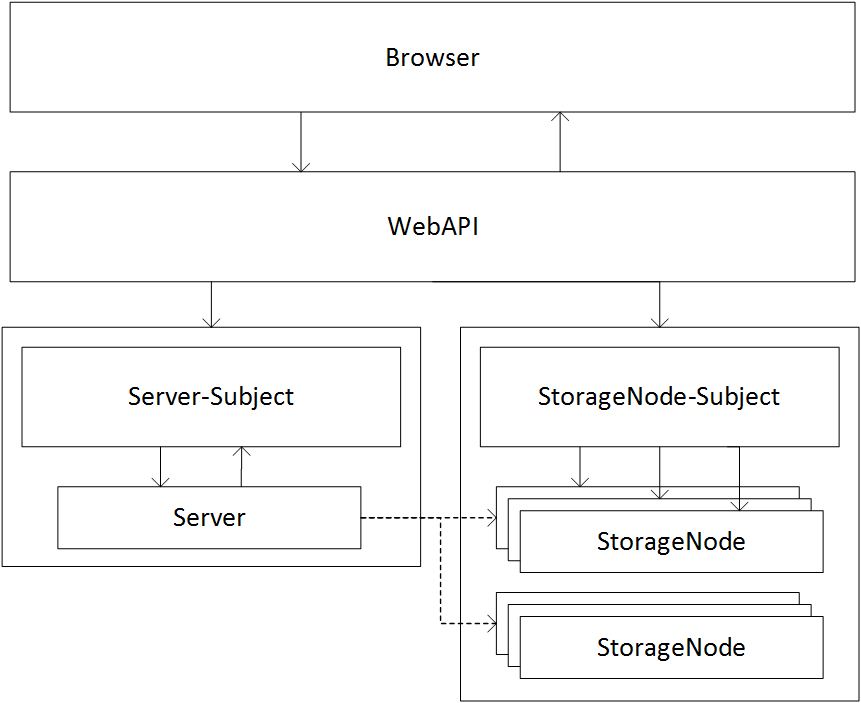
\includegraphics[width=9cm]{architecture.png}
			\end{minipage}
		\end{figure}
	\end{frame}
	\subsection{Message-Pathing}
	\begin{frame}{Message-Pathing}
		\begin{figure}
			\raggedright
			\begin{minipage}{1cm}
				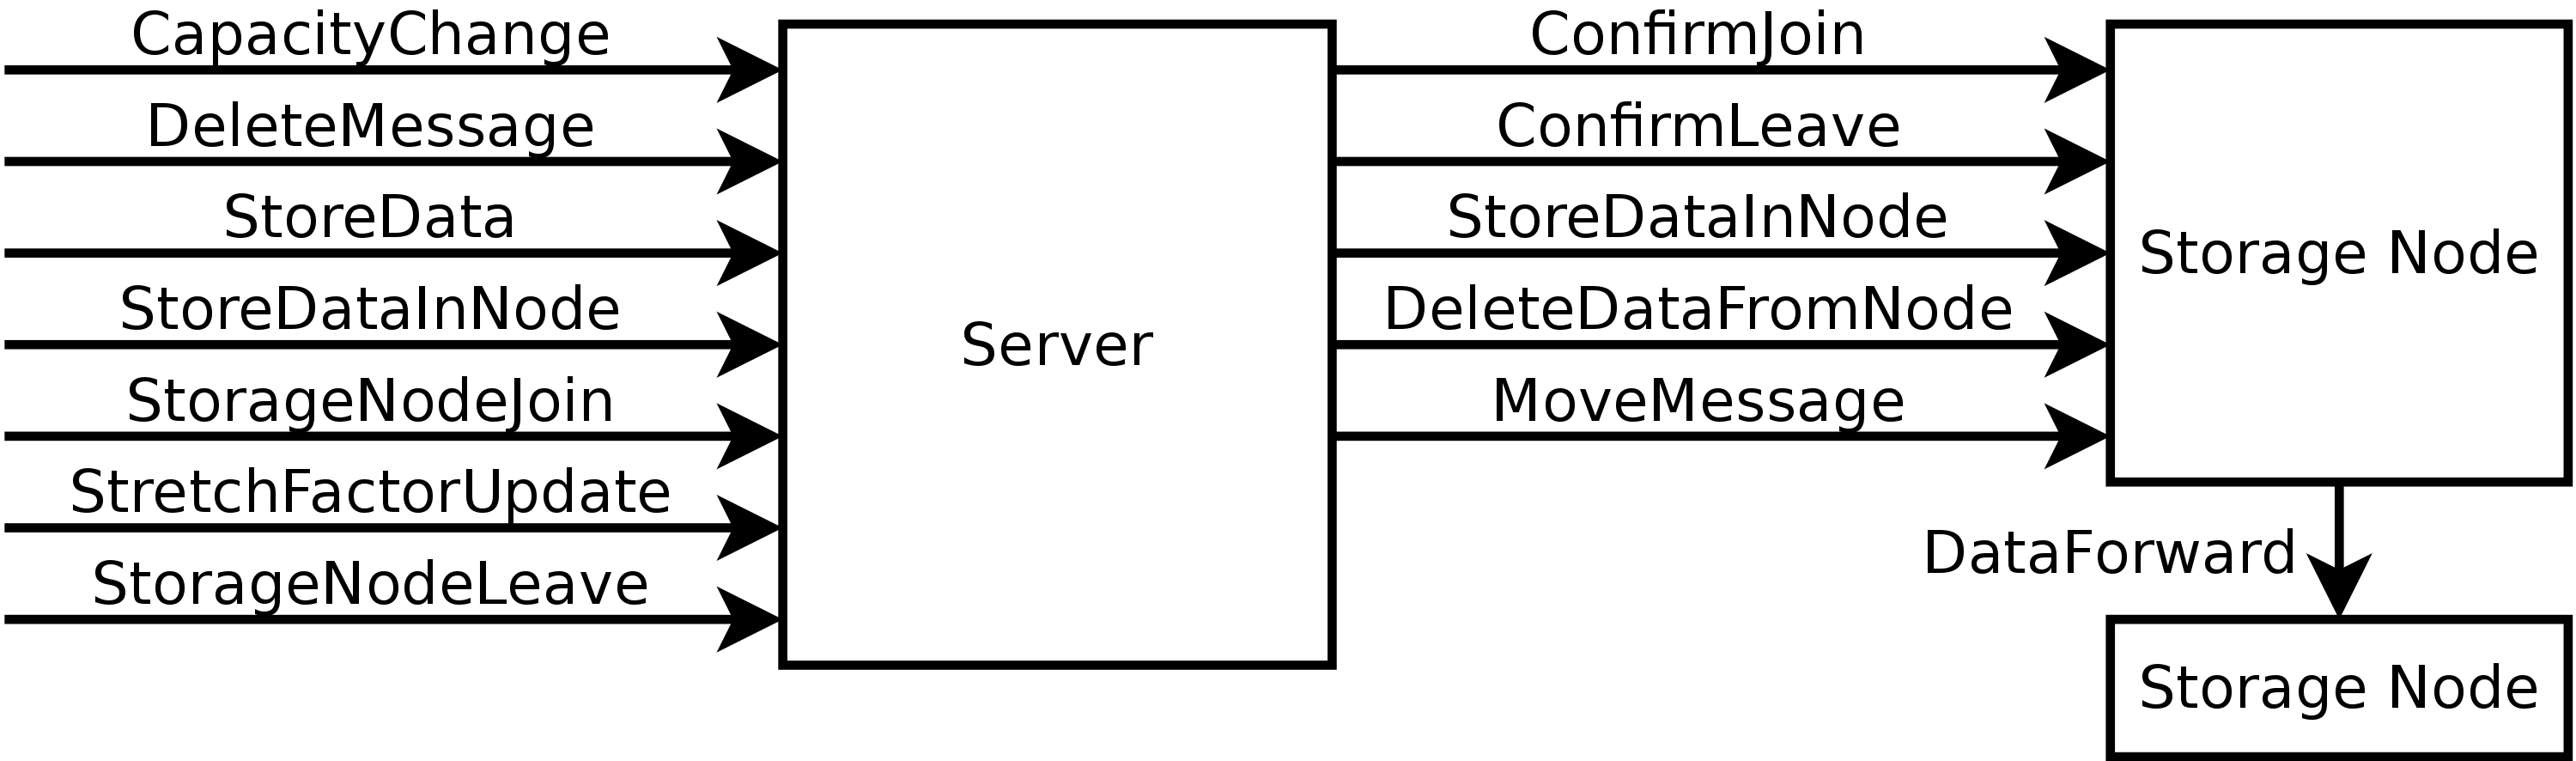
\includegraphics[width=10cm]{messages.png}
			\end{minipage}
		\end{figure}
	\end{frame}
	\subsection{Demo}
	\begin{frame}{Demo}
	\end{frame}
	\subsection{Resumé}
	\begin{frame}{Resumé}
	\end{frame}
	
\end{document}
